% --------------------------------------------------------------
% This is all preamble stuff that you don't have to worry about.
% Head down to where it says "Start here"
% --------------------------------------------------------------
 
\documentclass[12pt]{article}
 
\usepackage[margin=1in]{geometry}
\usepackage[alf, abnt-thesis-year=both]{abntex2cite}
\usepackage{microtype}          % para melhorias de justificação
\usepackage{morefloats}
\usepackage{enumitem}
\usepackage{amsmath,amsthm,amssymb}
\usepackage{subcaption}
\usepackage[table]{xcolor}
\usepackage{graphicx}
\usepackage{float}
 
\newcommand{\N}{\mathbb{N}}
\newcommand{\Z}{\mathbb{Z}}

\setlength{\arrayrulewidth}{1pt}
\setlength{\tabcolsep}{12pt}
\renewcommand{\arraystretch}{2}
 
\newenvironment{theorem}[2][Theorem]{\begin{trivlist}
\item[\hskip \labelsep {\bfseries #1}\hskip \labelsep {\bfseries #2.}]}{\end{trivlist}}
\newenvironment{lemma}[2][Lemma]{\begin{trivlist}
\item[\hskip \labelsep {\bfseries #1}\hskip \labelsep {\bfseries #2.}]}{\end{trivlist}}
\newenvironment{exercise}[2][Exercise]{\begin{trivlist}
\item[\hskip \labelsep {\bfseries #1}\hskip \labelsep {\bfseries #2.}]}{\end{trivlist}}
\newenvironment{problem}[2][Problem]{\begin{trivlist}
\item[\hskip \labelsep {\bfseries #1}\hskip \labelsep {\bfseries #2.}]}{\end{trivlist}}
\newenvironment{question}[2][Question]{\begin{trivlist}
\item[\hskip \labelsep {\bfseries #1}\hskip \labelsep {\bfseries #2.}]}{\end{trivlist}}
\newenvironment{corollary}[2][Corollary]{\begin{trivlist}
\item[\hskip \labelsep {\bfseries #1}\hskip \labelsep {\bfseries #2.}]}{\end{trivlist}}

\newenvironment{solution}{\begin{proof}[Solution]}{\end{proof}}
 
\begin{document}
 
% --------------------------------------------------------------
%                         Start here
% --------------------------------------------------------------
 
\title{Projeto de Programação - Otimização de Algoritmos}
\author{Leandro Baêta Lustosa Pontes \\ Prof. Dr. Filipe Wall Mutz \\ Pesquisa em Computação Aplicada}
\date{IFES, Serra, 11/07/2020}

\maketitle

\section[Problema 1]{Problema 1}

Para o problema 1 observamos um empate técnico entre os algoritmos Hill-Climbing com restart e o Genetic Algorithm, ambos apresentaram resultados muitos contudentes e encontrando o mínimo global de -10, bem como o Simulated Annealing, no entanto esses dois tiveram 100\% das suas execuções terminando abaixo de -9, com um desvio padrão um pouco abaixo do 0.2. \\

Acredito que o Algoritmo Genético se destaque pela a sua inicialização, que leva ampla vantagem sobre os outros algoritmos, mas que eu entendo como um benefício do algoritmo. Para se ter uma ideia em quanto outros algoritmos iniciam com o valor da função objetivo próximo do máximo global, que é de 105.0366, enquanto o GA tem o seu gráfico de melhor valor, já iniciando abaixo de 0 é um contraste muito grande. Outra vantagem é a rápida convergência dos indivíduos da população para o mínimo global, podemos notar que isso ocorre em geral antes da iteração 100 como podemos verificar na figura \ref{fig:problema-1-genetic-algorithm-funcao-objetivo-best}. \\

O algoritmo Hill-Climbing com restart é muito eficiente em sua estratégia, pois a cada x iterações, nesse problema a cada 50 iterações ocorre um restart, e com esse reinício certas vezes de fato bem melhores do que as posições anteriores, outras vezes encontra melhores caminhos mesmo com um valor um pouco maior do que o anterior e por muitas vezes também verificamos valores muito piores do que os anteriores, como podemos verificar na figura \ref{fig:problema-1-hill-climbing-com-restart-funcao-objetivo-value}, mas é exatamente essa estratégia que dá tanto destaque para esse algoritmo. \\

O Simulated Annealing é um algoritmo nervoso que no início aceita muitos valores piores na perspectiva de encontrar um melhor ponto na busca por um mínimo global. Nas dez execuções encontramos apenas 2 valores acima de 0 e mesmo assim são valores muito próximos de 0, ou seja eles não ficaram tão presos a mínimos locais em relação a esse problema. Mas aqui como no Hill-Climbing com restart, vale o destaque para o gráfico de variação do valor atual, para notarmos o quão volátil é até a iteração 810/820 como podemos verificar na figura \ref{fig:problema-1-simulated-annealing-funcao-objetivo-value}. \\

O algoritmo Hill-Climbing apresenta grande velocidade na sua execução, pois é um algoritmo bem simples, com as pertubações nos dados sendo geradas com um desvio padrão de 2.0, para esse problema de minimização, verificamos que a maioria das execuções tendem a ficar abaixo de zero e cerca de metade das execuções conseguiram um resultado bem próximo do mínimo global, que é -10. Mas também notamos que muitas vezes o algoritmo fica preso em mínimos locais, nesse último estudo que usamos como referência foram 4 execuções que ficaram presas, com destaque para o valor máximo de 37.798.

\subsection{Algoritmo Hill-Climbing}

\begin{figure}[H]
\centering
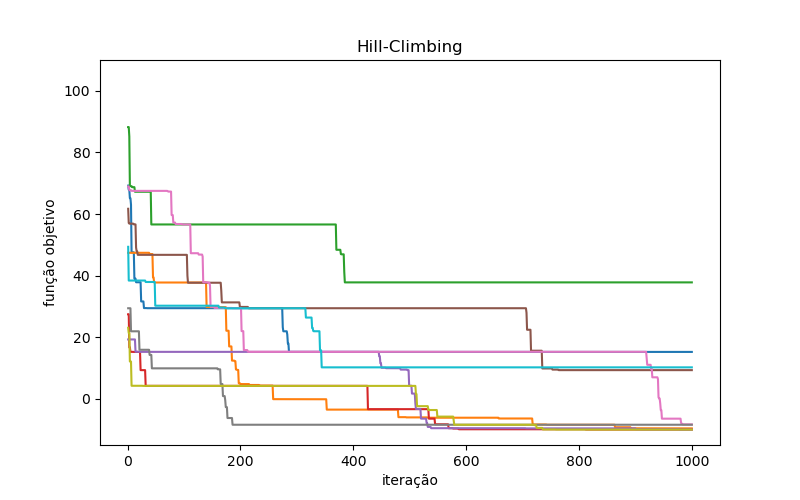
\includegraphics[width=110mm]{imagens/otima/problema-1-hill-climbing-funcao-objetivo-best.png}
\caption{Dados da execução da função objetivo durante as 10 iterações.
\label{fig:problema-1-hill-climbing-funcao-objetivo}}
\end{figure}

\subsection{Algoritmo Hill-Climbing com Restart}

\begin{figure}[H]
\centering
  \begin{minipage}[b]{0.48\textwidth}
    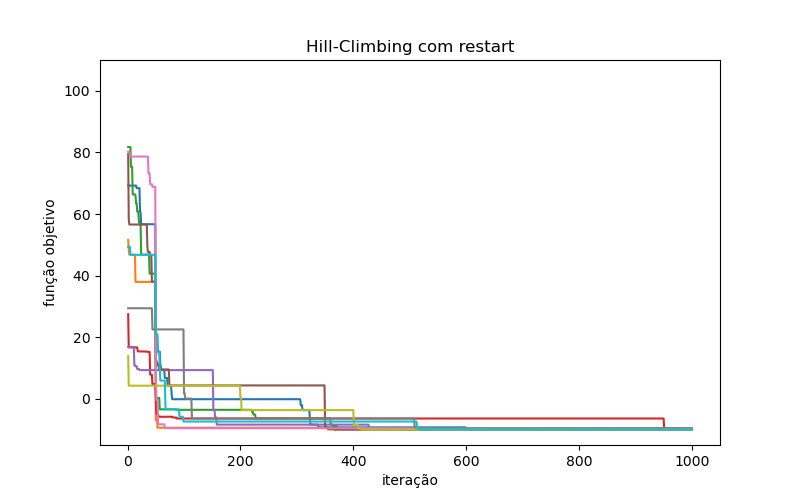
\includegraphics[width=88mm]{imagens/otima/problema-1-hill-climbing-com-restart-funcao-objetivo-best.png}
    \caption{Dados da execução da função objetivo durante as 10 iterações por melhor valor.
    \label{fig:problema-1-hill-climbing-com-restart-funcao-objetivo-best}}
  \end{minipage}
  \hfill
  \begin{minipage}[b]{0.48\textwidth}
    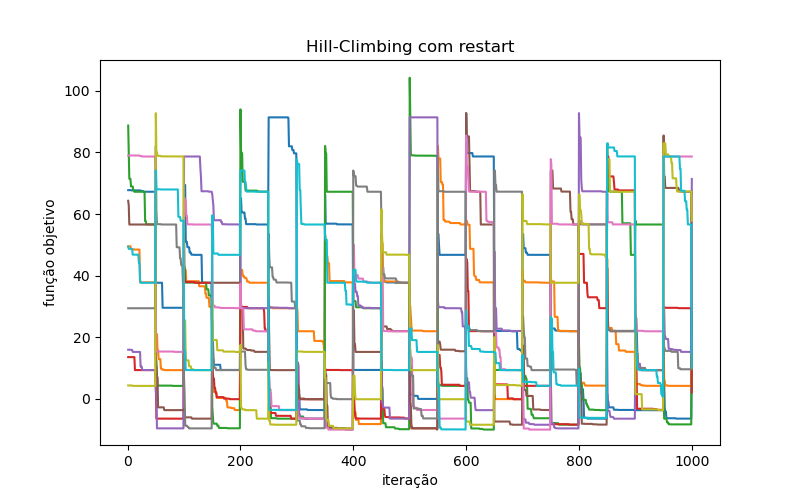
\includegraphics[width=88mm]{imagens/otima/problema-1-hill-climbing-com-restart-funcao-objetivo-value.png}
    \caption{Dados da execução da função objetivo durante as 10 iterações por valor atual.
    \label{fig:problema-1-hill-climbing-com-restart-funcao-objetivo-value}}
  \end{minipage}
\end{figure}

\subsection{Simulated Annealing}

\begin{figure}[H]
\centering
  \begin{minipage}[b]{0.48\textwidth}
    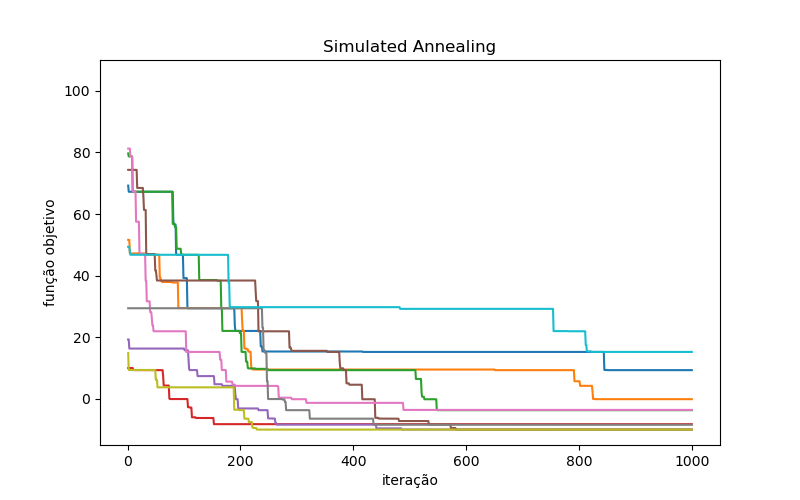
\includegraphics[width=88mm]{imagens/otima/problema-1-simulated-annealing-funcao-objetivo-best.png}
    \caption{Dados da execução da função objetivo durante as 10 iterações por melhor valor.
    \label{fig:problema-1-simulated-annealing-funcao-objetivo-best}}
  \end{minipage}
  \hfill
  \begin{minipage}[b]{0.48\textwidth}
    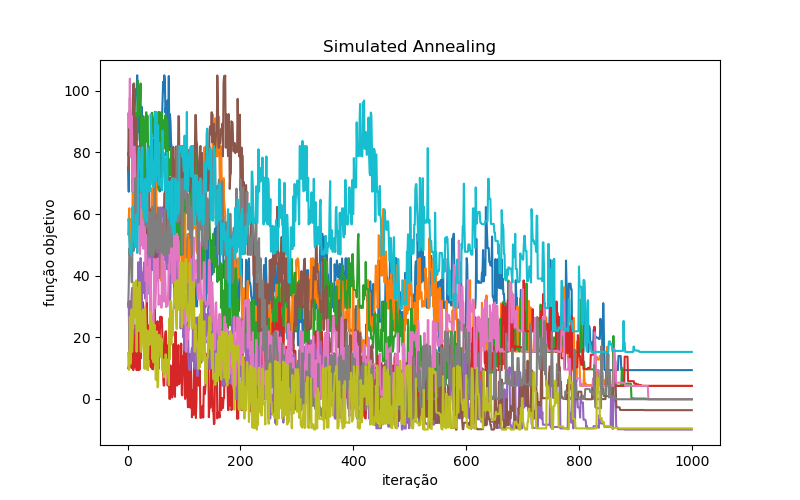
\includegraphics[width=88mm]{imagens/otima/problema-1-simulated-annealing-funcao-objetivo-value.png}
    \caption{Dados da execução da função objetivo durante as 10 iterações por valor atual.
    \label{fig:problema-1-simulated-annealing-funcao-objetivo-value}}
  \end{minipage}
\end{figure}

\subsection{Algoritmo Genético}

\begin{figure}[H]
\centering
  \begin{minipage}[b]{0.48\textwidth}
    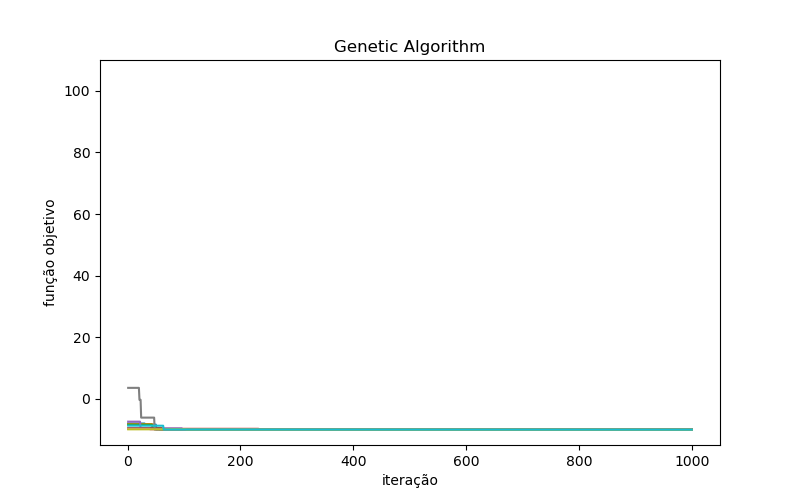
\includegraphics[width=88mm]{imagens/otima/problema-1-genetic-algorithm-funcao-objetivo-best.png}
    \caption{Dados da execução da função objetivo durante as 10 iterações por melhor valor.
    \label{fig:problema-1-genetic-algorithm-funcao-objetivo-best}}
  \end{minipage}
  \hfill
  \begin{minipage}[b]{0.48\textwidth}
    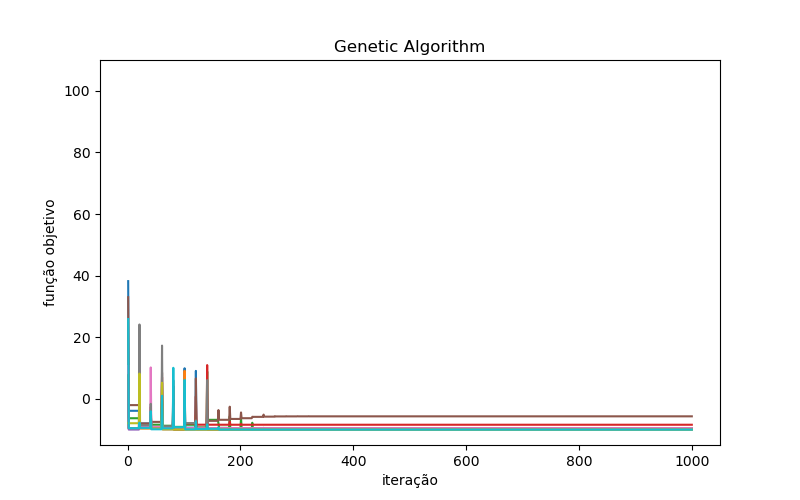
\includegraphics[width=88mm]{imagens/otima/problema-1-genetic-algorithm-funcao-objetivo-value.png}
    \caption{Dados da execução da função objetivo durante as 10 iterações por valor atual.
    \label{fig:problema-1-genetic-algorithm-funcao-objetivo-value}}
  \end{minipage}
\end{figure}
\subsection{Resumo}

\begin{table}[h!]
\centering
\begin{tabular}{ |c|c|c|c|c|  }
\hline
\rowcolor{lightgray}
Algoritmo & Max & Min & Média & Desvio Padrão \\
\hline
Hill-Climbing & 37.798 & -9.992 & 1.623 & 16.181 \\
\hline
Hill-Climbing com restart & -9.589 & -10.0 & -9.91 & 0.169 \\
\hline
Simulated Annealing & 4.3 & -10.0 & -6.245 & 5.463 \\
\hline
Genetic Algorithm & -9.606 & -10.0 & -9.878 & 0.188 \\
\hline

\end{tabular}
\caption{Tabela com dados consolidados dos algoritmos}
\end{table}

\begin{figure}[H]
\centering
  \begin{minipage}[b]{0.48\textwidth}
    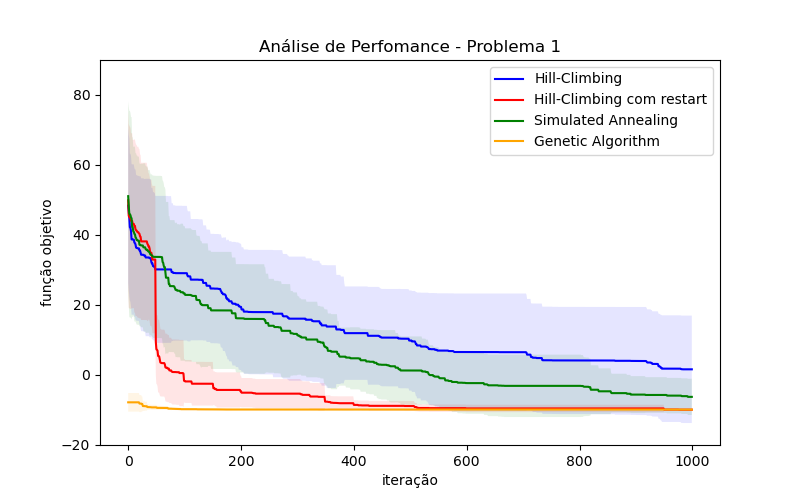
\includegraphics[width=88mm]{imagens/otima/problema-1-performance-algoritmos-best.png}
    \caption{Dados da execução da função objetivo durante as 10 iterações por melhor valor.
    \label{fig:problema-1-performance-algoritmos-best}}
  \end{minipage}
  \hfill
  \begin{minipage}[b]{0.48\textwidth}
    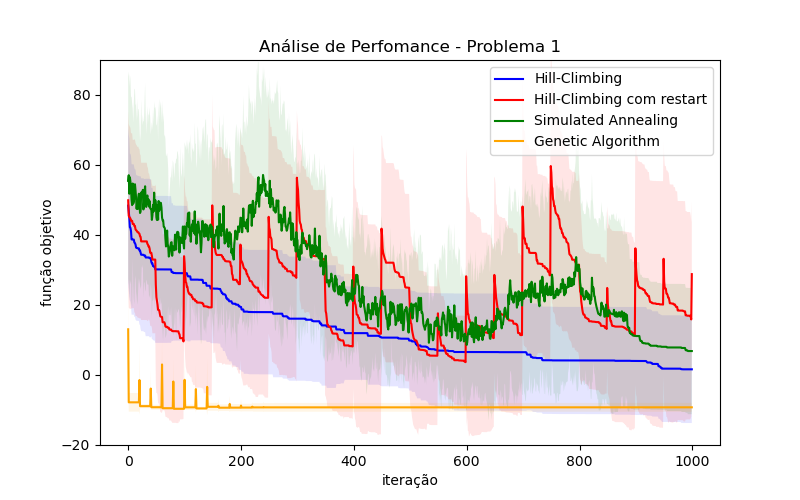
\includegraphics[width=88mm]{imagens/otima/problema-1-performance-algoritmos-value.png}
    \caption{Dados da execução da função objetivo durante as 10 iterações por valor atual.
    \label{fig:problema-1-performance-algoritmos-value}}
  \end{minipage}
\end{figure}
\section[Problema 2]{Problema 2}

Nesse problema tivemos uma situação um pouco diferente, pois podemos observar uma rápida convergência de todos os algoritmos para o mínimo global, isso pode ser notado nas figuras \ref{fig:problema-1-genetic-algorithm-funcao-objetivo-best}, \ref{fig:problema-1-hill-climbing-com-restart-funcao-objetivo-best}, \ref{fig:problema-1-hill-climbing-funcao-objetivo} e \ref{fig:problema-1-simulated-annealing-funcao-objetivo-best}. Eu acredito que isso tenha ocorrido pela distribuição dos valores iniciais para esse problema, mas também verifica-se que os valores das funções variam muito mesmo com vizinhos próximos, diferentemente do que ocorre com o problema anterior. Logo, para esse problema vamos declarar que os 4 algoritmos se destacaram e tiveram resultados muito próximos do mínimo global. \\

O algoritmo Hill-Climbing apresentou uma escalada muito abrupta já nas primeiras iterações e um pouco antes das 200 iterações encontrou alguns mínimos locais, já abaixo de 5 e que persistiram até quase o final da sua execução. \\

O algoritmo Hill-Climbing com restart teve a sua execução muito pareceida com o Hill-Climbing, diferença essa que só se vê nos detalhes e na apreciação do gráfico basado em valores atuais visto na figura \ref{fig:problema-2-hill-climbing-com-restart-funcao-objetivo-value}. \\

O algoritmo Simulated Annealing teve uma curva ainda mais acentuada, antes mesmo da iteração 100 o algoritmo já estava bem próximo dos mínimos globais, como pode ser visto na figura \ref{fig:problema-1-simulated-annealing-funcao-objetivo-best}. Mas algo que se destacou no Simulated Annealing foram os picos máximos observados próximos das iterações 400 e 600, onde o primeiro pico atingiu um valor próximo de 350 e o segundo 250, como pode ser visto na figura \ref{fig:problema-1-simulated-annealing-funcao-objetivo-value}. \\

O Algoritmo Genético apresenta grande similaridade com o Simulated Annealing no que se refere a rápida escalada, também encontrando valores próximos dos mínimos globais um pouco antes da iteração 100, como pode ser vista na figura \ref{fig:problema-2-genetic-algorithm-funcao-objetivo-best}.

\subsection{Algoritmo Hill-Climbing}

\begin{figure}[H]
\centering
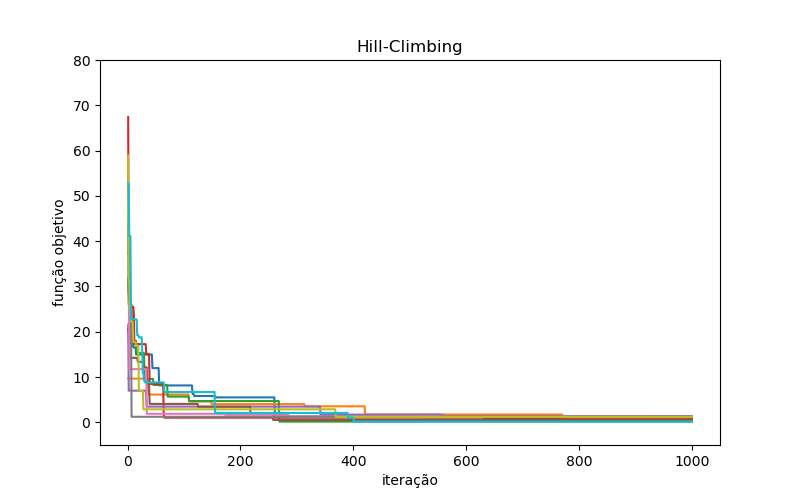
\includegraphics[width=110mm]{imagens/otima/problema-2-hill-climbing-funcao-objetivo-best.png}
\caption{Dados da execução da função objetivo durante as 10 iterações.
\label{fig:problema-2-hill-climbing-funcao-objetivo}}
\end{figure}

\subsection{Algoritmo Hill-Climbing com Restart}

\begin{figure}[H]
\centering
  \begin{minipage}[b]{0.48\textwidth}
    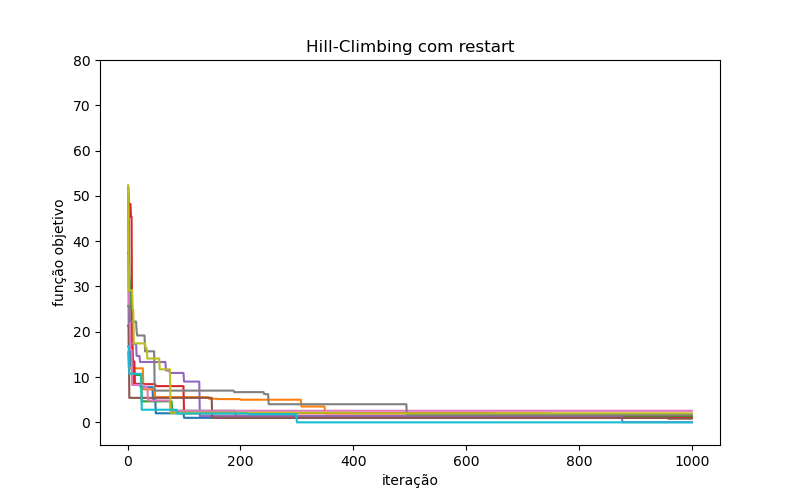
\includegraphics[width=88mm]{imagens/otima/problema-2-hill-climbing-com-restart-funcao-objetivo-best.png}
    \caption{Dados da execução da função objetivo durante as 10 iterações por melhor valor.
    \label{fig:problema-2-hill-climbing-com-restart-funcao-objetivo-best}}
  \end{minipage}
  \hfill
  \begin{minipage}[b]{0.48\textwidth}
    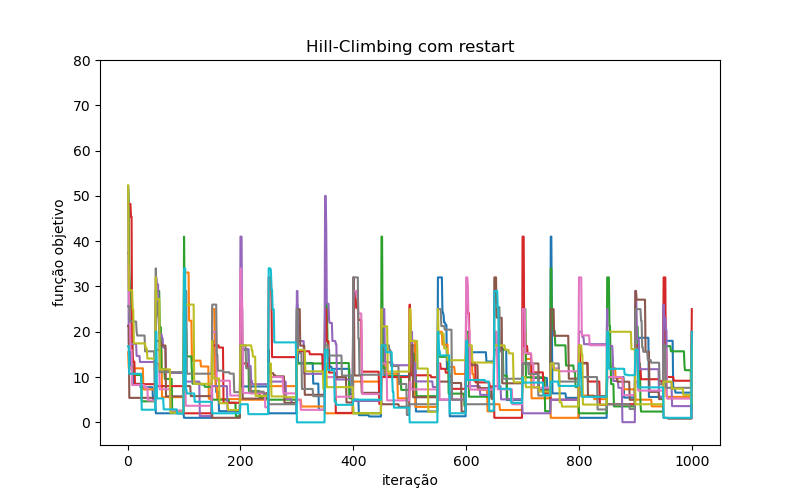
\includegraphics[width=88mm]{imagens/otima/problema-2-hill-climbing-com-restart-funcao-objetivo-value.png}
    \caption{Dados da execução da função objetivo durante as 10 iterações por valor atual.
    \label{fig:problema-2-hill-climbing-com-restart-funcao-objetivo-value}}
  \end{minipage}
\end{figure}

\subsection{Simulated Annealing}

\begin{figure}[H]
\centering
  \begin{minipage}[b]{0.48\textwidth}
    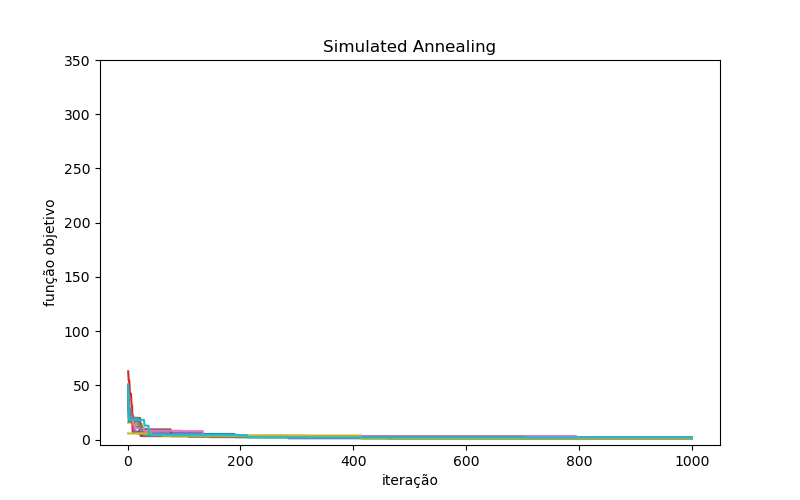
\includegraphics[width=88mm]{imagens/otima/problema-2-simulated-annealing-funcao-objetivo-best.png}
    \caption{Dados da execução da função objetivo durante as 10 iterações por melhor valor.
    \label{fig:problema-2-simulated-annealing-funcao-objetivo-best}}
  \end{minipage}
  \hfill
  \begin{minipage}[b]{0.48\textwidth}
    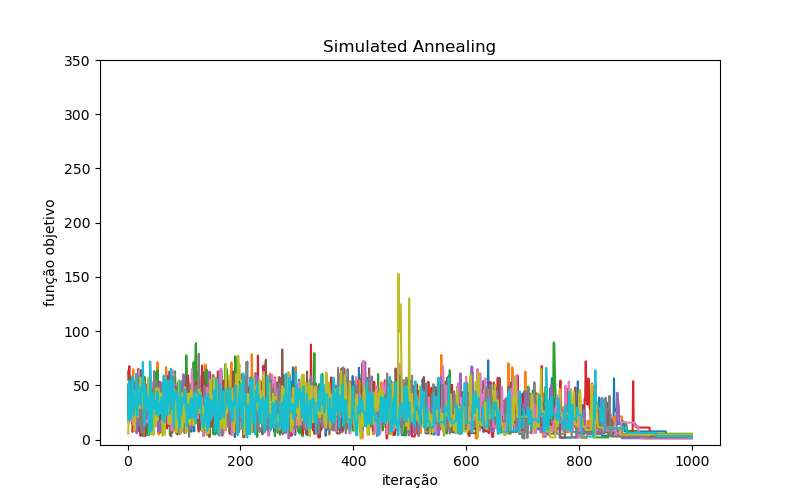
\includegraphics[width=88mm]{imagens/otima/problema-2-simulated-annealing-funcao-objetivo-value.png}
    \caption{Dados da execução da função objetivo durante as 10 iterações por valor atual.
    \label{fig:problema-2-simulated-annealing-funcao-objetivo-value}}
  \end{minipage}
\end{figure}

\subsection{Algoritmo Genético}

\begin{figure}[H]
\centering
  \begin{minipage}[b]{0.48\textwidth}
    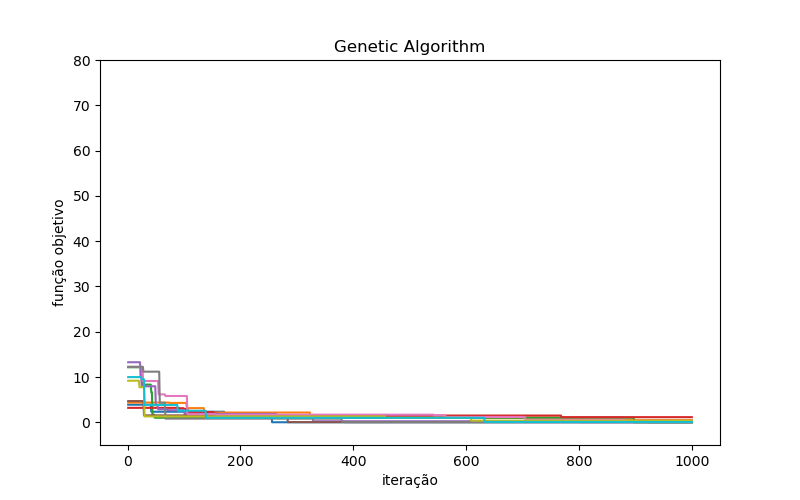
\includegraphics[width=88mm]{imagens/otima/problema-2-genetic-algorithm-funcao-objetivo-best.png}
    \caption{Dados da execução da função objetivo durante as 10 iterações por melhor valor.
    \label{fig:problema-2-genetic-algorithm-funcao-objetivo-best}}
  \end{minipage}
  \hfill
  \begin{minipage}[b]{0.48\textwidth}
    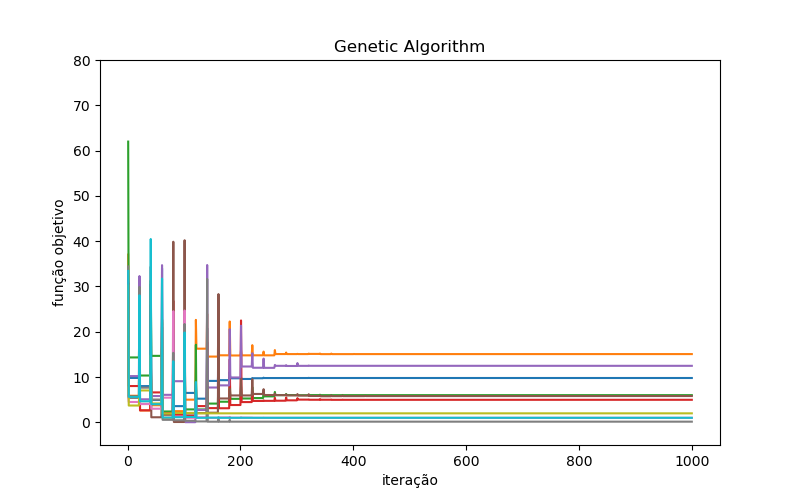
\includegraphics[width=88mm]{imagens/otima/problema-2-genetic-algorithm-funcao-objetivo-value.png}
    \caption{Dados da execução da função objetivo durante as 10 iterações por valor atual.
    \label{fig:problema-2-genetic-algorithm-funcao-objetivo-value}}
  \end{minipage}
\end{figure}
\subsection{Resumo}

\begin{table}[h!]
\centering
\begin{tabular}{ |c|c|c|c|c|  }
\hline
\rowcolor{lightgray}
Algoritmo & Max & Min & Média & Desvio Padrão \\
\hline
Hill-Climbing & 2.369 & 0.144 & 1.05 & 0.682 \\
\hline
Hill-Climbing com restart & 2.556 & 0.0 & 1.137 & 0.795 \\
\hline
Simulated Annealing & 3.089 & 0.546 & 1.48 & 0.711 \\
\hline
Genetic Algorithm & 1.949 & 0.037 & 1.027 & 0.737 \\
\hline

\end{tabular}
\caption{Tabela com dados consolidados dos algoritmos}
\end{table}

\begin{figure}[H]
\centering
  \begin{minipage}[b]{0.48\textwidth}
    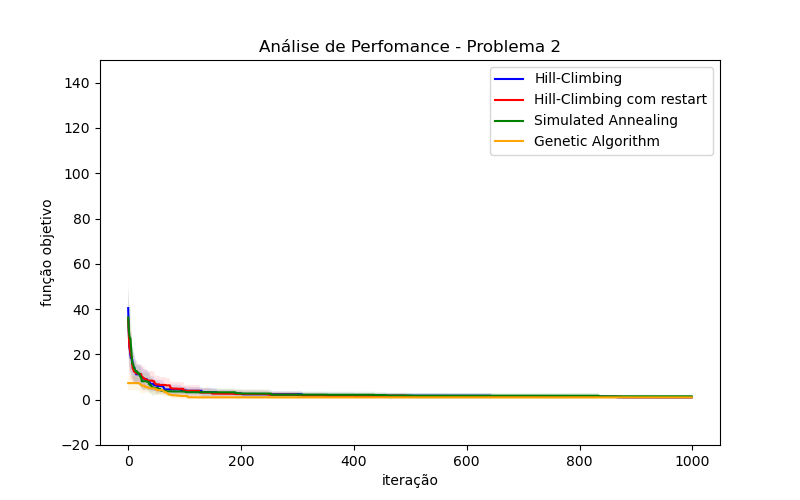
\includegraphics[width=88mm]{imagens/otima/problema-2-performance-algoritmos-best.png}
    \caption{Dados da execução da função objetivo durante as 10 iterações por melhor valor.
    \label{fig:problema-2-performance-algoritmos-best}}
  \end{minipage}
  \hfill
  \begin{minipage}[b]{0.48\textwidth}
    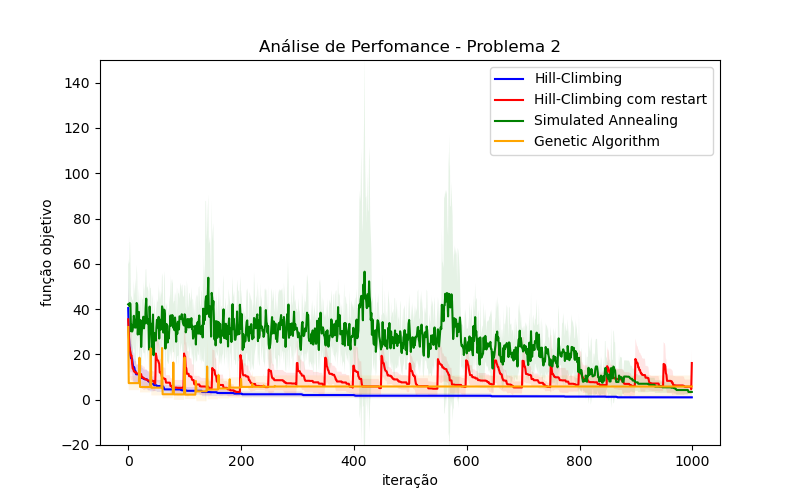
\includegraphics[width=88mm]{imagens/otima/problema-2-performance-algoritmos-value.png}
    \caption{Dados da execução da função objetivo durante as 10 iterações por valor atual.
    \label{fig:problema-2-performance-algoritmos-value}}
  \end{minipage}
\end{figure}
\section[Problema 3]{Problema 3}

Nesse problema do caxeiro viajante, o Algoritmo Genético se destacou, apresentando os melhores resultados entre todos os demais algoritmos, enquanto todos os demais ficaram presos no mínimo local próximo de 19000, o GA chegou alcançar o mínimo local de 15538, ainda que seja um valor muito longe do mínimo global, que é de 6656, observamos que esse algoritmo ainda não havia chegado ao seu potencial máximo, pois os valores de novas populações ainda estavam oscilando muito, como pode ser visto na figura \ref{fig:problema-3-genetic-algorithm-funcao-objetivo-value}, se compararmos com as figuras dos problemas anteriores \ref{fig:problema-1-genetic-algorithm-funcao-objetivo-value} e \ref{fig:problema-2-genetic-algorithm-funcao-objetivo-value}, vemos claramente que mesmo após 100k iterações os valores atuais ainda não haviam convergido para um valor único, enquanto nos demais problemas essa convergência ocorreu pouco após a iteração 200. \\

O algoritmo genético apesar de possuir um peso computacional muito elevado, apresentou uma eficiência muito maior em encontrar novos mínimos locais, acreditamos que após algumas análises sobre esse problema que a aplicação de algumas heurísticas para melhorar a eficácia não só desse mas de todos os demais seja um caminho mais adequado, por exemplo evitando que path's cruzem com outros, verificamos que em geral a rota que segue o perímetro mais externo dos pontos, possui a distância mais curta. \\

O algoritmo Hill-Climbing apresentou boa performance para esse problema e conseguiu ao longo das iterações fugir de mínimos locais. \\

Os algoritmos Hill-Climbing com restart e Simulated Annealing apresentaram um comportamento muito parecido com números muito similares também.

\subsection{Algoritmo Hill-Climbing}

\begin{figure}[H]
\centering
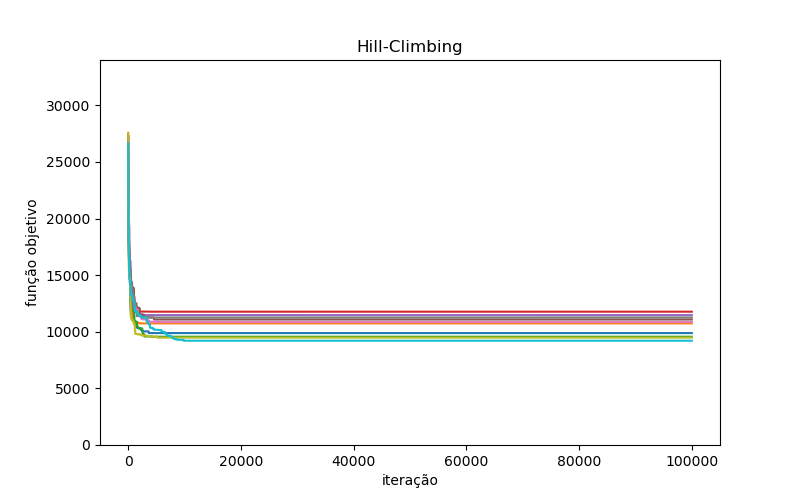
\includegraphics[width=110mm]{imagens/otima/problema-3-hill-climbing-funcao-objetivo-best.png}
\caption{Dados da execução da função objetivo durante as 10 iterações.
\label{fig:problema-3-hill-climbing-funcao-objetivo}}
\end{figure}

\subsection{Algoritmo Hill-Climbing com Restart}

\begin{figure}[H]
\centering
  \begin{minipage}[b]{0.48\textwidth}
    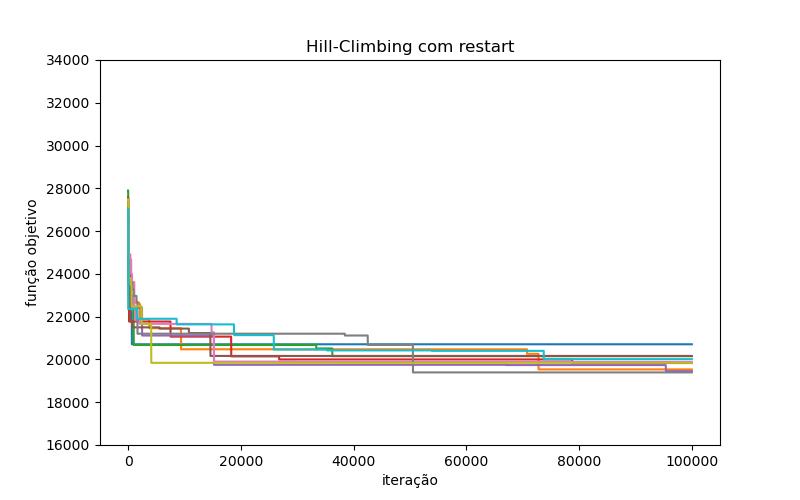
\includegraphics[width=88mm]{imagens/otima/problema-3-hill-climbing-com-restart-funcao-objetivo-best.png}
    \caption{Dados da execução da função objetivo durante as 10 iterações por melhor valor.
    \label{fig:problema-3-hill-climbing-com-restart-funcao-objetivo-best}}
  \end{minipage}
  \hfill
  \begin{minipage}[b]{0.48\textwidth}
    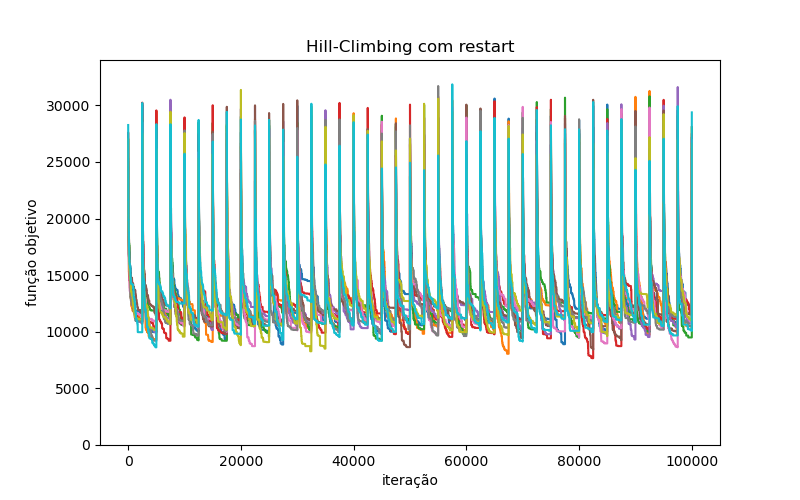
\includegraphics[width=88mm]{imagens/otima/problema-3-hill-climbing-com-restart-funcao-objetivo-value.png}
    \caption{Dados da execução da função objetivo durante as 10 iterações por valor atual.
    \label{fig:problema-3-hill-climbing-com-restart-funcao-objetivo-value}}
  \end{minipage}
\end{figure}

\subsection{Simulated Annealing}

\begin{figure}[H]
\centering
  \begin{minipage}[b]{0.48\textwidth}
    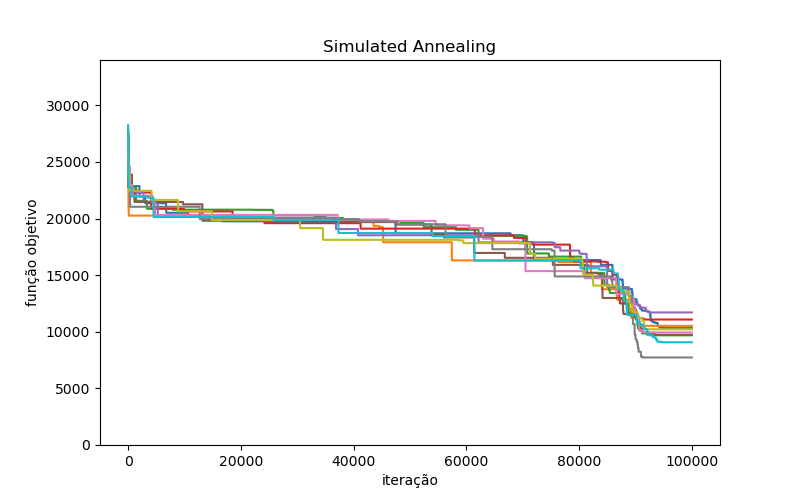
\includegraphics[width=88mm]{imagens/otima/problema-3-simulated-annealing-funcao-objetivo-best.png}
    \caption{Dados da execução da função objetivo durante as 10 iterações por melhor valor.
    \label{fig:problema-3-simulated-annealing-funcao-objetivo-best}}
  \end{minipage}
  \hfill
  \begin{minipage}[b]{0.48\textwidth}
    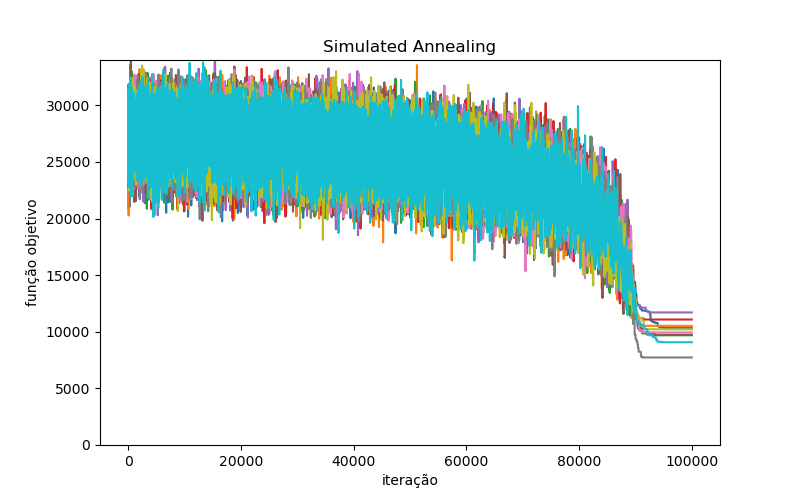
\includegraphics[width=88mm]{imagens/otima/problema-3-simulated-annealing-funcao-objetivo-value.png}
    \caption{Dados da execução da função objetivo durante as 10 iterações por valor atual.
    \label{fig:problema-3-simulated-annealing-funcao-objetivo-value}}
  \end{minipage}
\end{figure}

\subsection{Algoritmo Genético}

\begin{figure}[H]
\centering
  \begin{minipage}[b]{0.48\textwidth}
    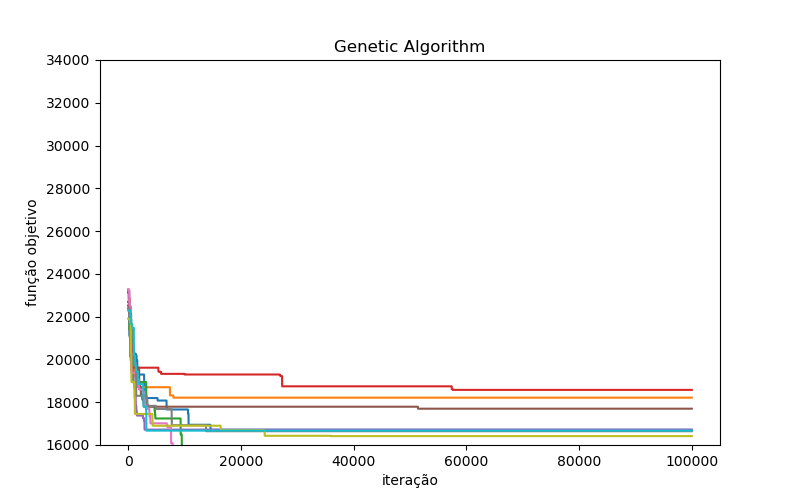
\includegraphics[width=88mm]{imagens/otima/problema-3-genetic-algorithm-funcao-objetivo-best.png}
    \caption{Dados da execução da função objetivo durante as 10 iterações por melhor valor.
    \label{fig:problema-3-genetic-algorithm-funcao-objetivo-best}}
  \end{minipage}
  \hfill
  \begin{minipage}[b]{0.48\textwidth}
    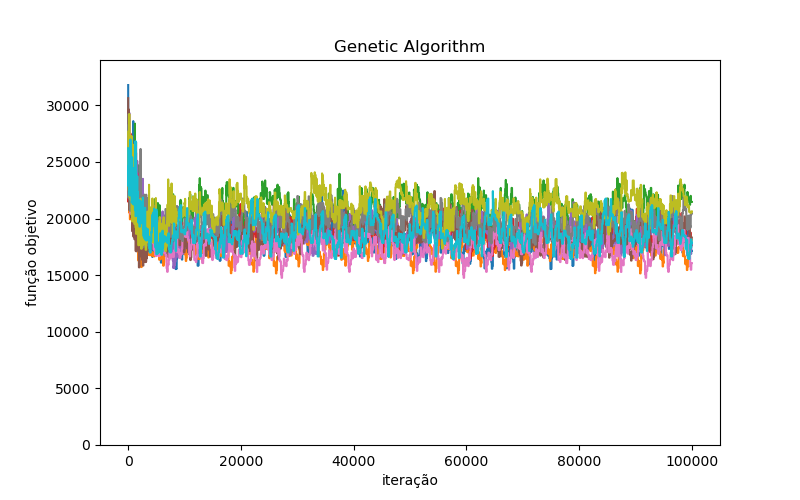
\includegraphics[width=88mm]{imagens/otima/problema-3-genetic-algorithm-funcao-objetivo-value.png}
    \caption{Dados da execução da função objetivo durante as 10 iterações por valor atual.
    \label{fig:problema-3-genetic-algorithm-funcao-objetivo-value}}
  \end{minipage}
\end{figure}
\subsection{Resumo}

\begin{table}[h!]
\centering
\begin{tabular}{ |c|c|c|c|c|  }
\hline
\rowcolor{lightgray}
Algoritmo & Max & Min & Média & Desvio Padrão \\
\hline
Hill-Climbing & 11773.256 & 9209.255 & 10531.702 & 919.177 \\
\hline
Hill-Climbing com restart & 9316.101 & 7665.887 & 8626.72 & 539.401 \\
\hline
Simulated Annealing & 11707.327 & 7730.449 & 10000.987 & 1089.323 \\
\hline
Genetic Algorithm & 17478.514 & 15008.897 & 16138.323 & 883.279 \\
\hline

\end{tabular}
\caption{Tabela com dados consolidados dos algoritmos}
\end{table}

\begin{figure}[H]
\centering
  \begin{minipage}[b]{0.48\textwidth}
    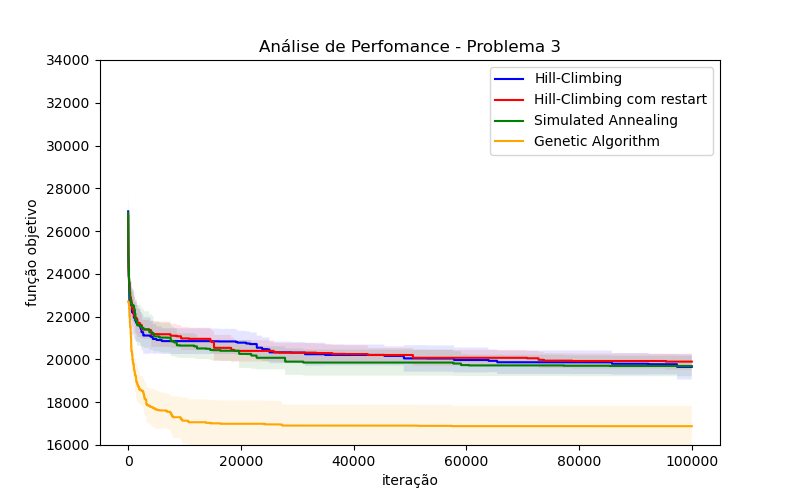
\includegraphics[width=88mm]{imagens/otima/problema-3-performance-algoritmos-best.png}
    \caption{Dados da execução da função objetivo durante as 10 iterações por melhor valor.
    \label{fig:problema-3-performance-algoritmos-best}}
  \end{minipage}
  \hfill
  \begin{minipage}[b]{0.48\textwidth}
    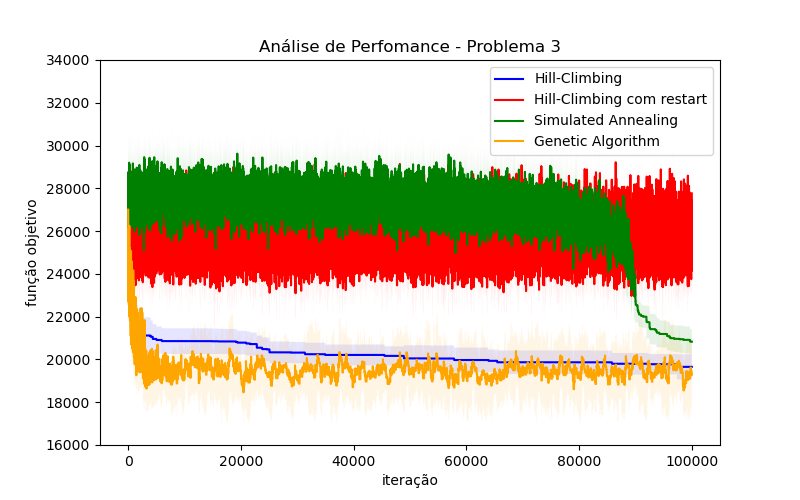
\includegraphics[width=88mm]{imagens/otima/problema-3-performance-algoritmos-value.png}
    \caption{Dados da execução da função objetivo durante as 10 iterações por valor atual.
    \label{fig:problema-3-performance-algoritmos-value}}
  \end{minipage}
\end{figure}

% --------------------------------------------------------------
%     You don't have to mess with anything below this line.
% --------------------------------------------------------------
 
\end{document}
